\documentclass[12pt, a4paper, oneside]{ctexart}
\usepackage{amsmath, amsthm, amssymb, appendix, bm, graphicx, hyperref, mathrsfs}
\usepackage{enumerate}
\usepackage{float}
\usepackage{booktabs} 
\usepackage{caption}
\usepackage{geometry}
\usepackage{algorithm}
\usepackage{algpseudocode}
\geometry{margin=1in}

\title{\textbf{聚类分析}}
\author{王一鑫}
\date{\today}
\linespread{1.5}
\newtheorem{theorem}{定理}[section]
\newtheorem{definition}[theorem]{定义}
\newtheorem{lemma}[theorem]{引理}
\newtheorem{corollary}[theorem]{推论}
\newtheorem{example}[theorem]{例}
\newtheorem{proposition}[theorem]{命题}
\renewcommand{\abstractname}{\Large\textbf{摘要}}
\usepackage{listings}
\usepackage{xcolor}
\definecolor{mygreen}{rgb}{0,0.6,0}
\definecolor{mygray}{rgb}{0.5,0.5,0.5}
\definecolor{mymauve}{rgb}{0.58,0,0.82}


\lstset{numbers=left, %设置行号位置
	numberstyle=\tiny\color{mygray}, %设置行号大小
	basicstyle=\footnotesize,
	keywordstyle=\color{blue}, %设置关键字颜色
	commentstyle=\color{mygreen}, %设置注释颜色
	frame=single, %设置边框格式
	rulecolor=\color{black},
	escapeinside=``, %逃逸字符(1左面的键),用于显示中文
	%breaklines, %自动折行
	extendedchars=false, %解决代码跨页时,章节标题,页眉等汉字不显示的问题
	xleftmargin=2em,xrightmargin=2em, aboveskip=1em, %设置边距
	tabsize=2, %设置tab空格数
	showspaces=false,%不显示空格
	breaklines=true,  
	stringstyle=\color{orange}
}


\begin{document}
	
	\maketitle
	
	\setcounter{page}{0}
	\maketitle
	\thispagestyle{empty}
	
	\begin{abstract} 
		本文围绕K均值聚类算法在实际数据分析中的应用展开,系统介绍了K均值聚类的数学原理、优化目标函数及其实现算法. 首先介绍了K均值聚类算法,以及通过肘部法确定聚类数的原理与公式推导;其次,以英国罗马统治时期五个窑口出土陶器的化学成分数据为例,结合散点图矩阵、方差分析和主成分分析(PCA)对数据进行了预处理和结构可视化. 通过PCA降维观察发现样本具有明显聚类趋势,并进一步利用K均值算法进行分类. 聚类结果显示三个类别与窑口地理分布具有一致性,验证了K均值方法在考古类数据中的实际适用性与解释力.
		
		\par\textbf{关键词:} 聚类分析;K均值算法;主成分分析
	\end{abstract}
		
	\newpage
	\pagenumbering{Roman}
	\setcounter{page}{1}
	\tableofcontents
	\newpage
	\setcounter{page}{1}
	\pagenumbering{arabic}
	
	\section{聚类分析}
	
	\subsection{问题背景}
	聚类分析(clustering)是在一个数据集中寻找子群或类的多元统计分析方法. 将一些个体分类是人类具有的必不可少的能力,从婴儿开始,就学着分辨各种事物. 同样一些事物, 可以分成不同的类别. 比如,图书可以按学科分类,也可以按封面图案分类,显然学科分类更有用. 一副扑克牌,可以按花色分类,可以按点数分类,可以按有无人物分类. 所谓的“类”,通俗来讲就是相似元素的集合.
	
	在聚类分析中,根据分类的对象不同,可分为两类:R-型聚类分析和 Q-型聚类分析,其中 R-型是对变量或指标进行分类,Q-型是对样本进行分类。在进行 R-型和 Q-型聚类分析时,常通过距离和相似系数进行聚类.
	
	聚类分析在机器学习领域又称为无监督学习,这是因为数据中并没有现成的分类可供参考. 而回归分析、判别分析方法则称为有监督学习.
	
	常用的聚类分析方法有
	\begin{enumerate}[(1)]
		\item 系统(谱系)聚类法(hierarchical clustering),从每类只有单个元素开始,每次合并两类;
		\item k均值聚类法(k-means clustering),需要设定类的个数,然后迭代地调整元素的类属使同类的元素接近而异类元素分离.
		\item 基于统计模型的方法,如混合密度模型.
	\end{enumerate}
	本文主要实现K均值聚类法.
	\subsection{K均值聚类法}
	$K$均值聚类($K$-mean clustering)是把数据集分成$K$个不重复的简单快捷的统计方法,是聚类分析中的经典算法. 在进行$K$均值聚类分析时,首先要确定聚类个数$K$的大小,然后$K$均值聚类算法将会把每个样本观测准确地分配到$K$个类中.
	
	令$G_1, G_2, \dots, G_K$分别表示在每个类中包含观测样本的集合,并要求它们满足下面两个性质:
	
	\begin{enumerate}[(1)]
		\item $G_1 \cup G_2 \cup \cdots \cup G_K = \{1, \dots, n\}$,即每个观测样本属于$K$个类中至少一个类;
		\item 对每个 $k \ne l$,都有 $G_k \cap G_l = \emptyset$. 表示没有一个观测样本同时属于两个类或更多的类中.
	\end{enumerate}
	
	$K$均值聚类的核心思想是:好的聚类方法使同类内所有数据点的总体差异性尽可能小. 令$W(G_k)$表示第$k$类$G_k$的类内差异性度量值,$K$均值聚类方法主要是通过极小化下面的目标函数,找到最优的类$G_1, G_2, \cdots, G_K$,即
	
	\begin{equation}
		\min_{G_1, \dots, G_K} \left\{ \sum_{k=1}^{K} W(G_k) \right\}.
		\label{WGK}
	\end{equation}
	
	式 \eqref{WGK} 是把所有样本观测值分到$K$个类中,使得$K$个类总的类内差异性尽可能小.为了解极小化目标函数 \eqref{WGK} ,首先需要定义类内差异性$W(G_k)$.
	
	简单起见,采用最常用的平方欧氏距离,即
	\begin{equation}
		W(G_k) = \frac{1}{|G_k|} \sum_{i,i' \in G_k} \sum_{j=1}^{p} (x_{ij} - x_{i'j})^2, \quad k = 1, \cdots, K,
		\label{SquareEuclideanDistance}
	\end{equation}
	
	其中 $|G_k|$ 表示 $G_k$ 类中观测样本的数量. 由式 \eqref{WGK} 和式 \eqref{SquareEuclideanDistance} ,$K$ 均值聚类方法可求解下面的最优化问题:
	
	\begin{equation}
		\min_{G_1, \cdots, G_K} \left\{ \sum_{k=1}^{K} \frac{1}{|G_k|} \sum_{i,i' \in G_k} \sum_{j=1}^{p} (x_{ij} - x_{i'j})^2 \right\}.
		\label{Kmeans}
	\end{equation}
	
	现在需要一种快速的优化算法来求解上面的最小化问题 \eqref{Kmeans},为了解决该问题并减少计算量,可以考虑下面的局部最优的 $K$ 均值聚类算法.
	\begin{algorithm}
		\caption{K-means 聚类算法}
		\begin{algorithmic}[1]
			\Require 样本数据集 $X = \{x_1, x_2, \dots, x_n\}$,聚类数目 $K$
			\Ensure 每个样本所属的类标记
			\State \textbf{初始化}:对每个样本随机分配一个从 $1$ 到 $K$ 的初始类别
			\Repeat
			\For{每个类 $k = 1$ 到 $K$}
			\State 计算第 $k$ 类的类中心 $\mu_k$,为该类样本在各维度的均值向量
			\EndFor
			\For{每个样本 $x_i$}
			\State 计算 $x_i$ 到所有类中心 $\mu_k$ 的平方欧氏距离
			\State 将 $x_i$ 分配给距离最近的类
			\EndFor
			\Until{样本类别不再发生变化}
		\end{algorithmic}
	\end{algorithm}
	
	当聚类结果不再发生变化时,分类就达到了一个局部最优解. K均值聚类算法的结果未必是全局最优解,依赖于不同初值.
	
	k 均值法需要预先确定类的个数,但是完全可以选择一个类数的范围,对每一个类个数运行算法,然后基于某种准则选择一个类个数. 比如,当增加类个数时类内离差平方和减少幅度明显变小时,就不再增加类个数.
	
	k 方法是各种软件中常见的聚类方法,最适用于各类的个数相近,空间形状接近凸集的情形. 如果真实类别的成员个数有很大差别,用k方法可能会将大的类拆分;如果真实类别的空间形状不是球形或者椭球形,用k某某方法的效果可能也不好.
	
	\subsection{K均值聚类中类的个数}
	K均值聚类方法的一个确定是需要事先确定一个K,实际应用中非常困难,本节介绍基于类内平方和变化的方法确定类的个数K.
	
	\begin{definition}
		定义WSS(组内平方距离之和为
		\begin{equation}
			\mathrm{WSS}_k = \sum_{\ell=1}^{k} \sum_{x_i \in C_\ell} d^2(x_i, \bar{x}_\ell)
			\label{WSS1}
		\end{equation}
		
	\end{definition}
	
	其中 $k$ 是类的个数,$C_\ell$ 表示第 $\ell$ 个类的观测集合,$\bar{x}_\ell$ 是第 $\ell$ 个类的重心.
	
	可以在不同的 $k$ 之间比较 $\mathrm{WSS}_k$ 的值,当然,分类越多这个值越小,$\mathrm{WSS}_k$ 是 $k$ 的减函数,在其减少很快的时候应继续多分类,但是减少很慢的时候就不应该继续分类了,找到这样的“拐点”就可以确定类的个数. 这种方法成为肘方法(elbow method).
	
	$\mathrm{WSS}_k$ 的另一种等价定义是:
	
	\begin{equation}
		\mathrm{WSS}_k = \sum_{\ell=1}^{k} \frac{1}{2n_\ell} \sum_{x_i \in C_\ell} \sum_{x_j \in C_\ell} d^2(x_i, x_j)
		\label{WSS2}
	\end{equation}
	\subsection{实例分析:陶器考古聚类}
	\begin{example}
		数据集pottery包含了对罗马统治时期英国的5个窑出土的陶器的化学测量数据. 对这5个窑处于的地区进行聚类分析.
	\end{example}
	读取数据集:
	\begin{lstlisting}[language=R]
		library(GGally)
		library(HSAUR2)
		library(tidyr)
		library(dplyr)
		library(forcats)
		data("pottery", package = "HSAUR2")
	\end{lstlisting}
	
	绘制散点图矩阵,结果见图 \ref{fig:scatter_matrix}.
	\begin{lstlisting}[language=R]
		## 散点图矩阵
		p1 <- ggscatmat(
		data = pottery,
		columns = 1:9, color = "kiln"
		)
	\end{lstlisting}
	\begin{figure}[H]
		\centering
		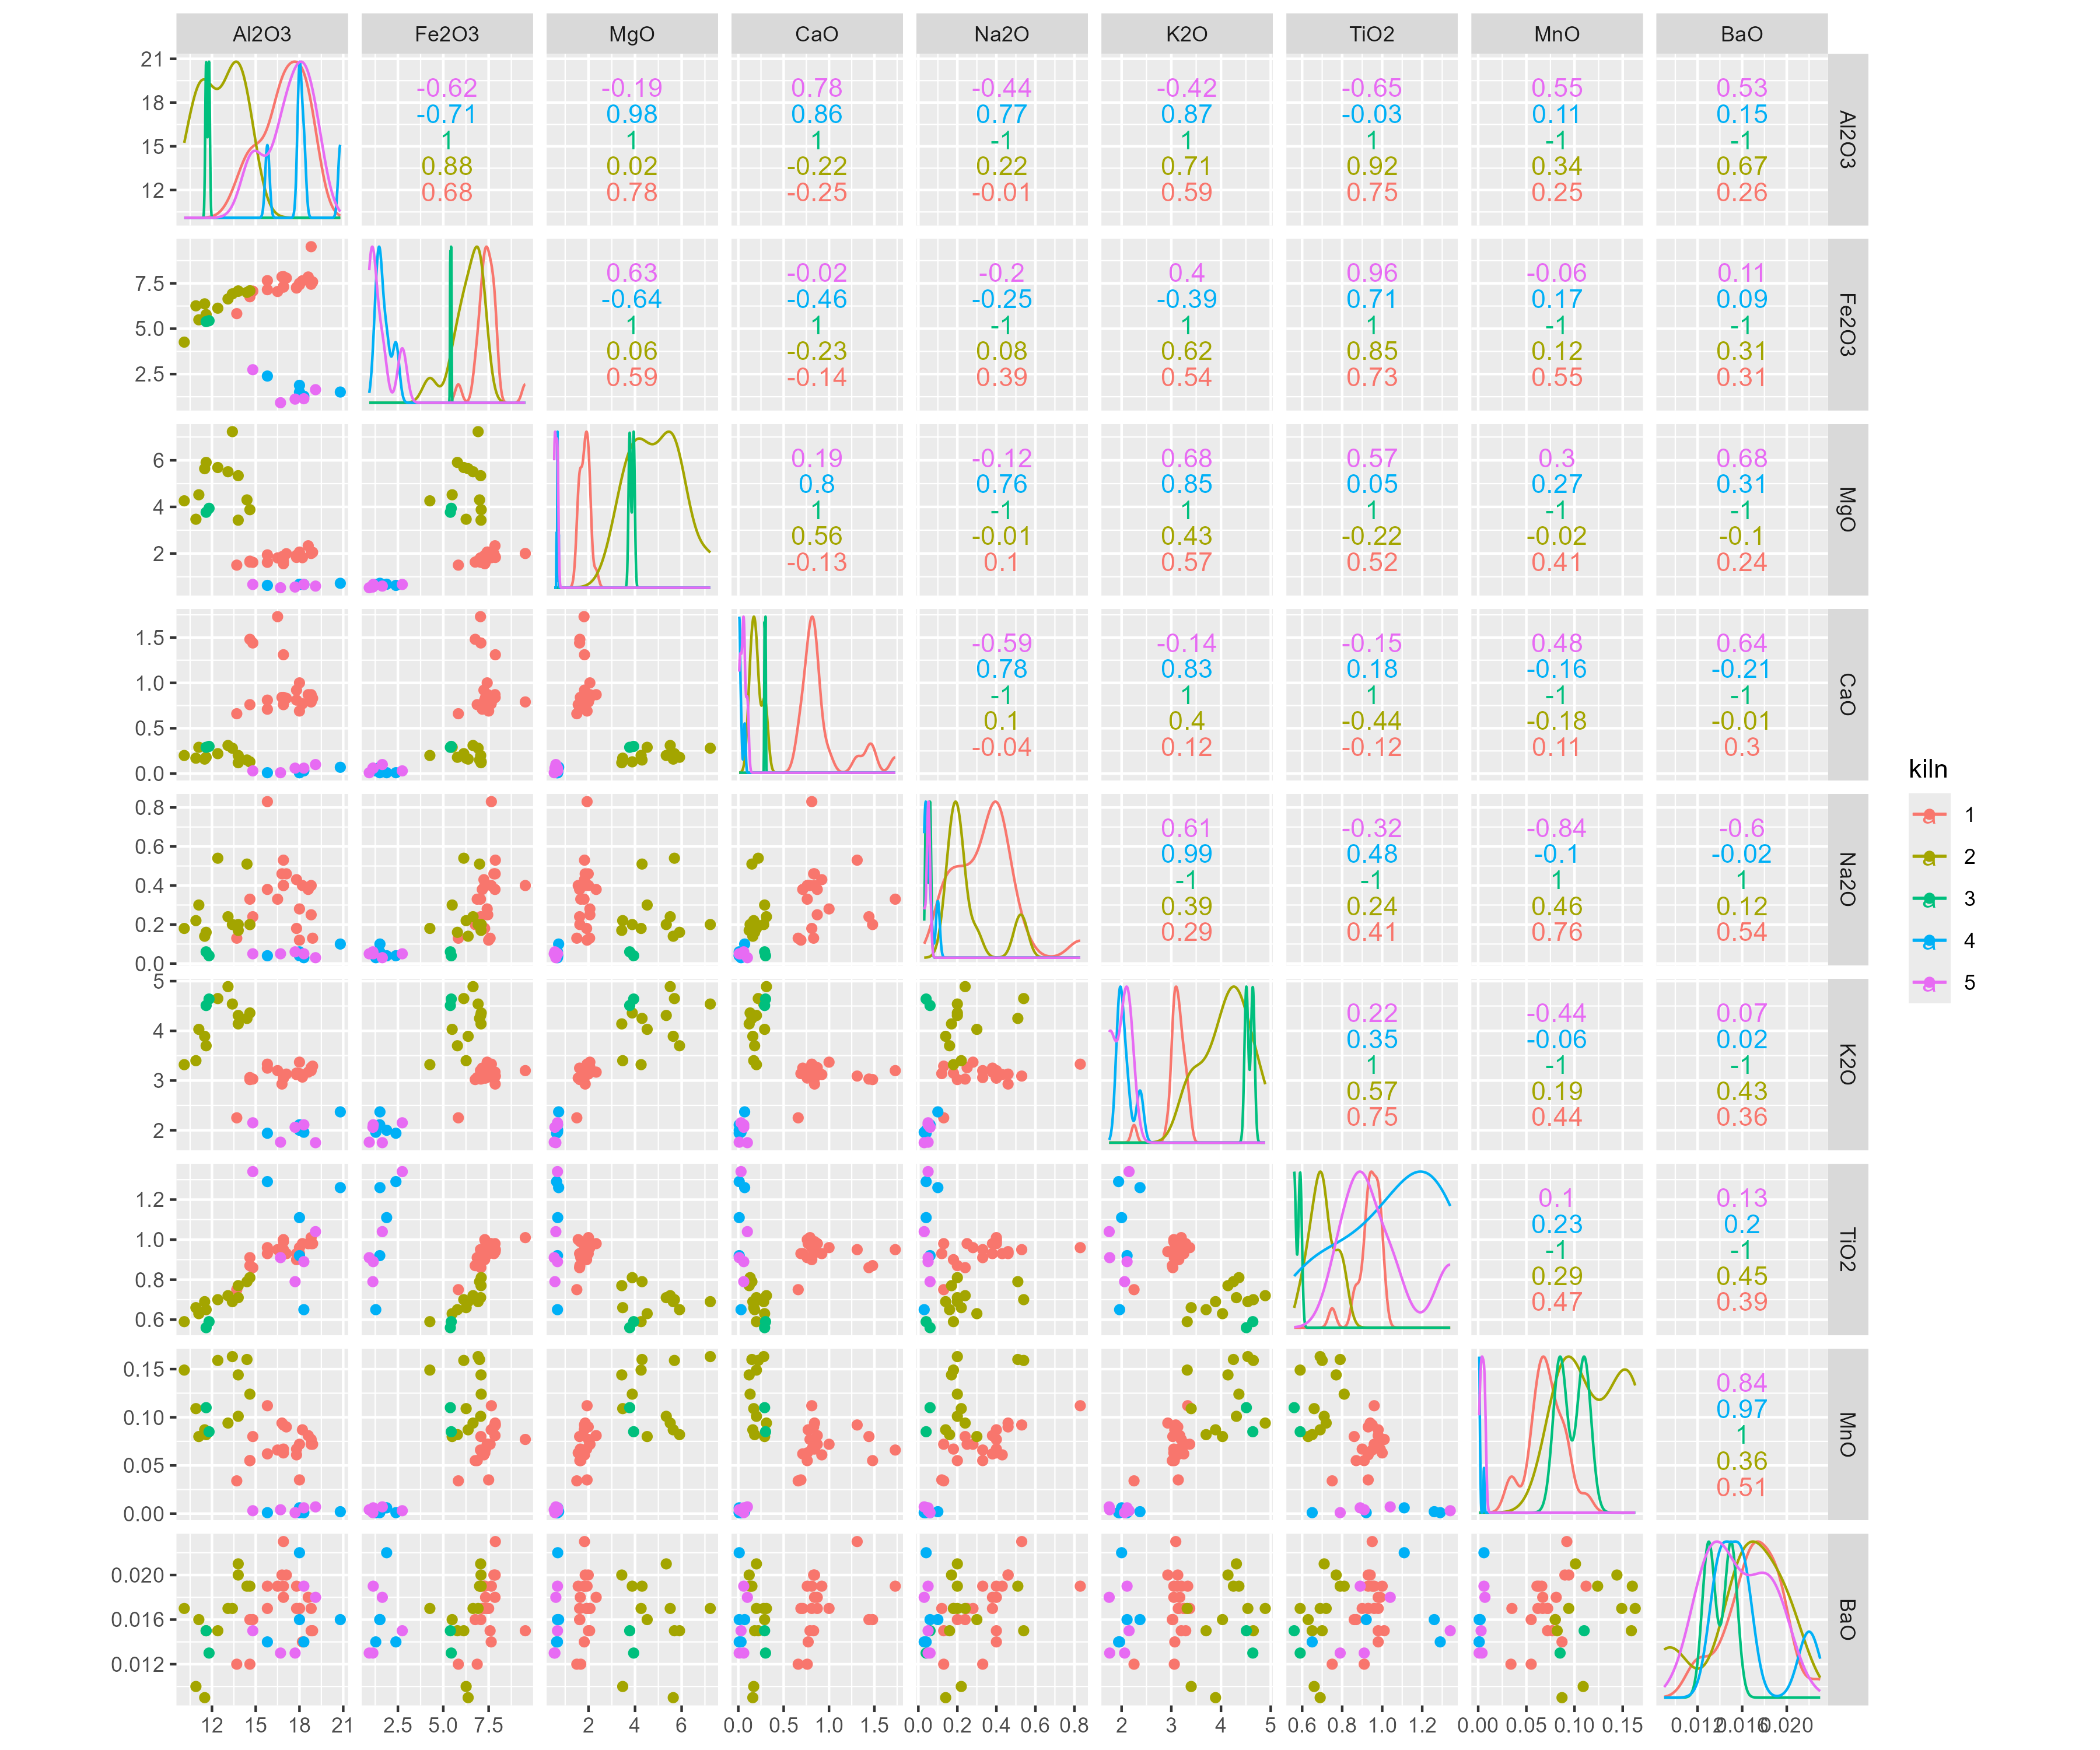
\includegraphics[width=0.8\textwidth]{../Figure/scatter_matrix.png}
		\caption{陶器样本各化学成分的散点图矩阵}
		\label{fig:scatter_matrix}
	\end{figure}
	
	计算各个变量的方差,见表 \ref{table:Variance}.
	\begin{lstlisting}[language=R]
		## 各个变量的方差
		var_tbl <- pottery |>
		summarise(across(
		-kiln, var
		)) |>
		pivot_longer(everything(),
		names_to = "Chemical",
		values_to = "Var"
		)
	\end{lstlisting}
	\begin{table}[htbp]
		\centering
		\caption{各个变量的方差}
		\label{table:Variance}
		\begin{tabular}{lr}
			\toprule
			Chemical & Var \\
			\midrule
			Al2O3 & 7.3063 \\
			Fe2O3 & 5.7879 \\
			MgO & 3.0349 \\
			CaO & 0.2064 \\
			Na2O & 0.0318 \\
			\addlinespace
			K2O & 0.7271 \\
			TiO2 & 0.0323 \\
			MnO & 0.0022 \\
			BaO & 0.0000 \\
			\bottomrule
		\end{tabular}
	\end{table}
	
	由于方差的差别较大,应进行标准化.
	\begin{lstlisting}[language=R]
		## 标准化处理
		pottery_scale <- pottery |>
		mutate(across(-kiln, \(x) (x - mean(x)) / sd(x)))
	\end{lstlisting}
	
	应对高维数据,考虑降维方法主成分分析(PCA).基于相关阵计算主成分,作前两个主成分的散点图,见图 \ref{fig:PCA_kiln} .
	\begin{lstlisting}[language=R]
		as_tibble(pot_pca) |>
		mutate(kiln = pottery[["kiln"]]) |>
		ggplot(aes(
		x = Comp.1, y = Comp.2, color = kiln
		)) +
		geom_point() -> p2
	\end{lstlisting}
	\begin{figure}[H]
		\centering
		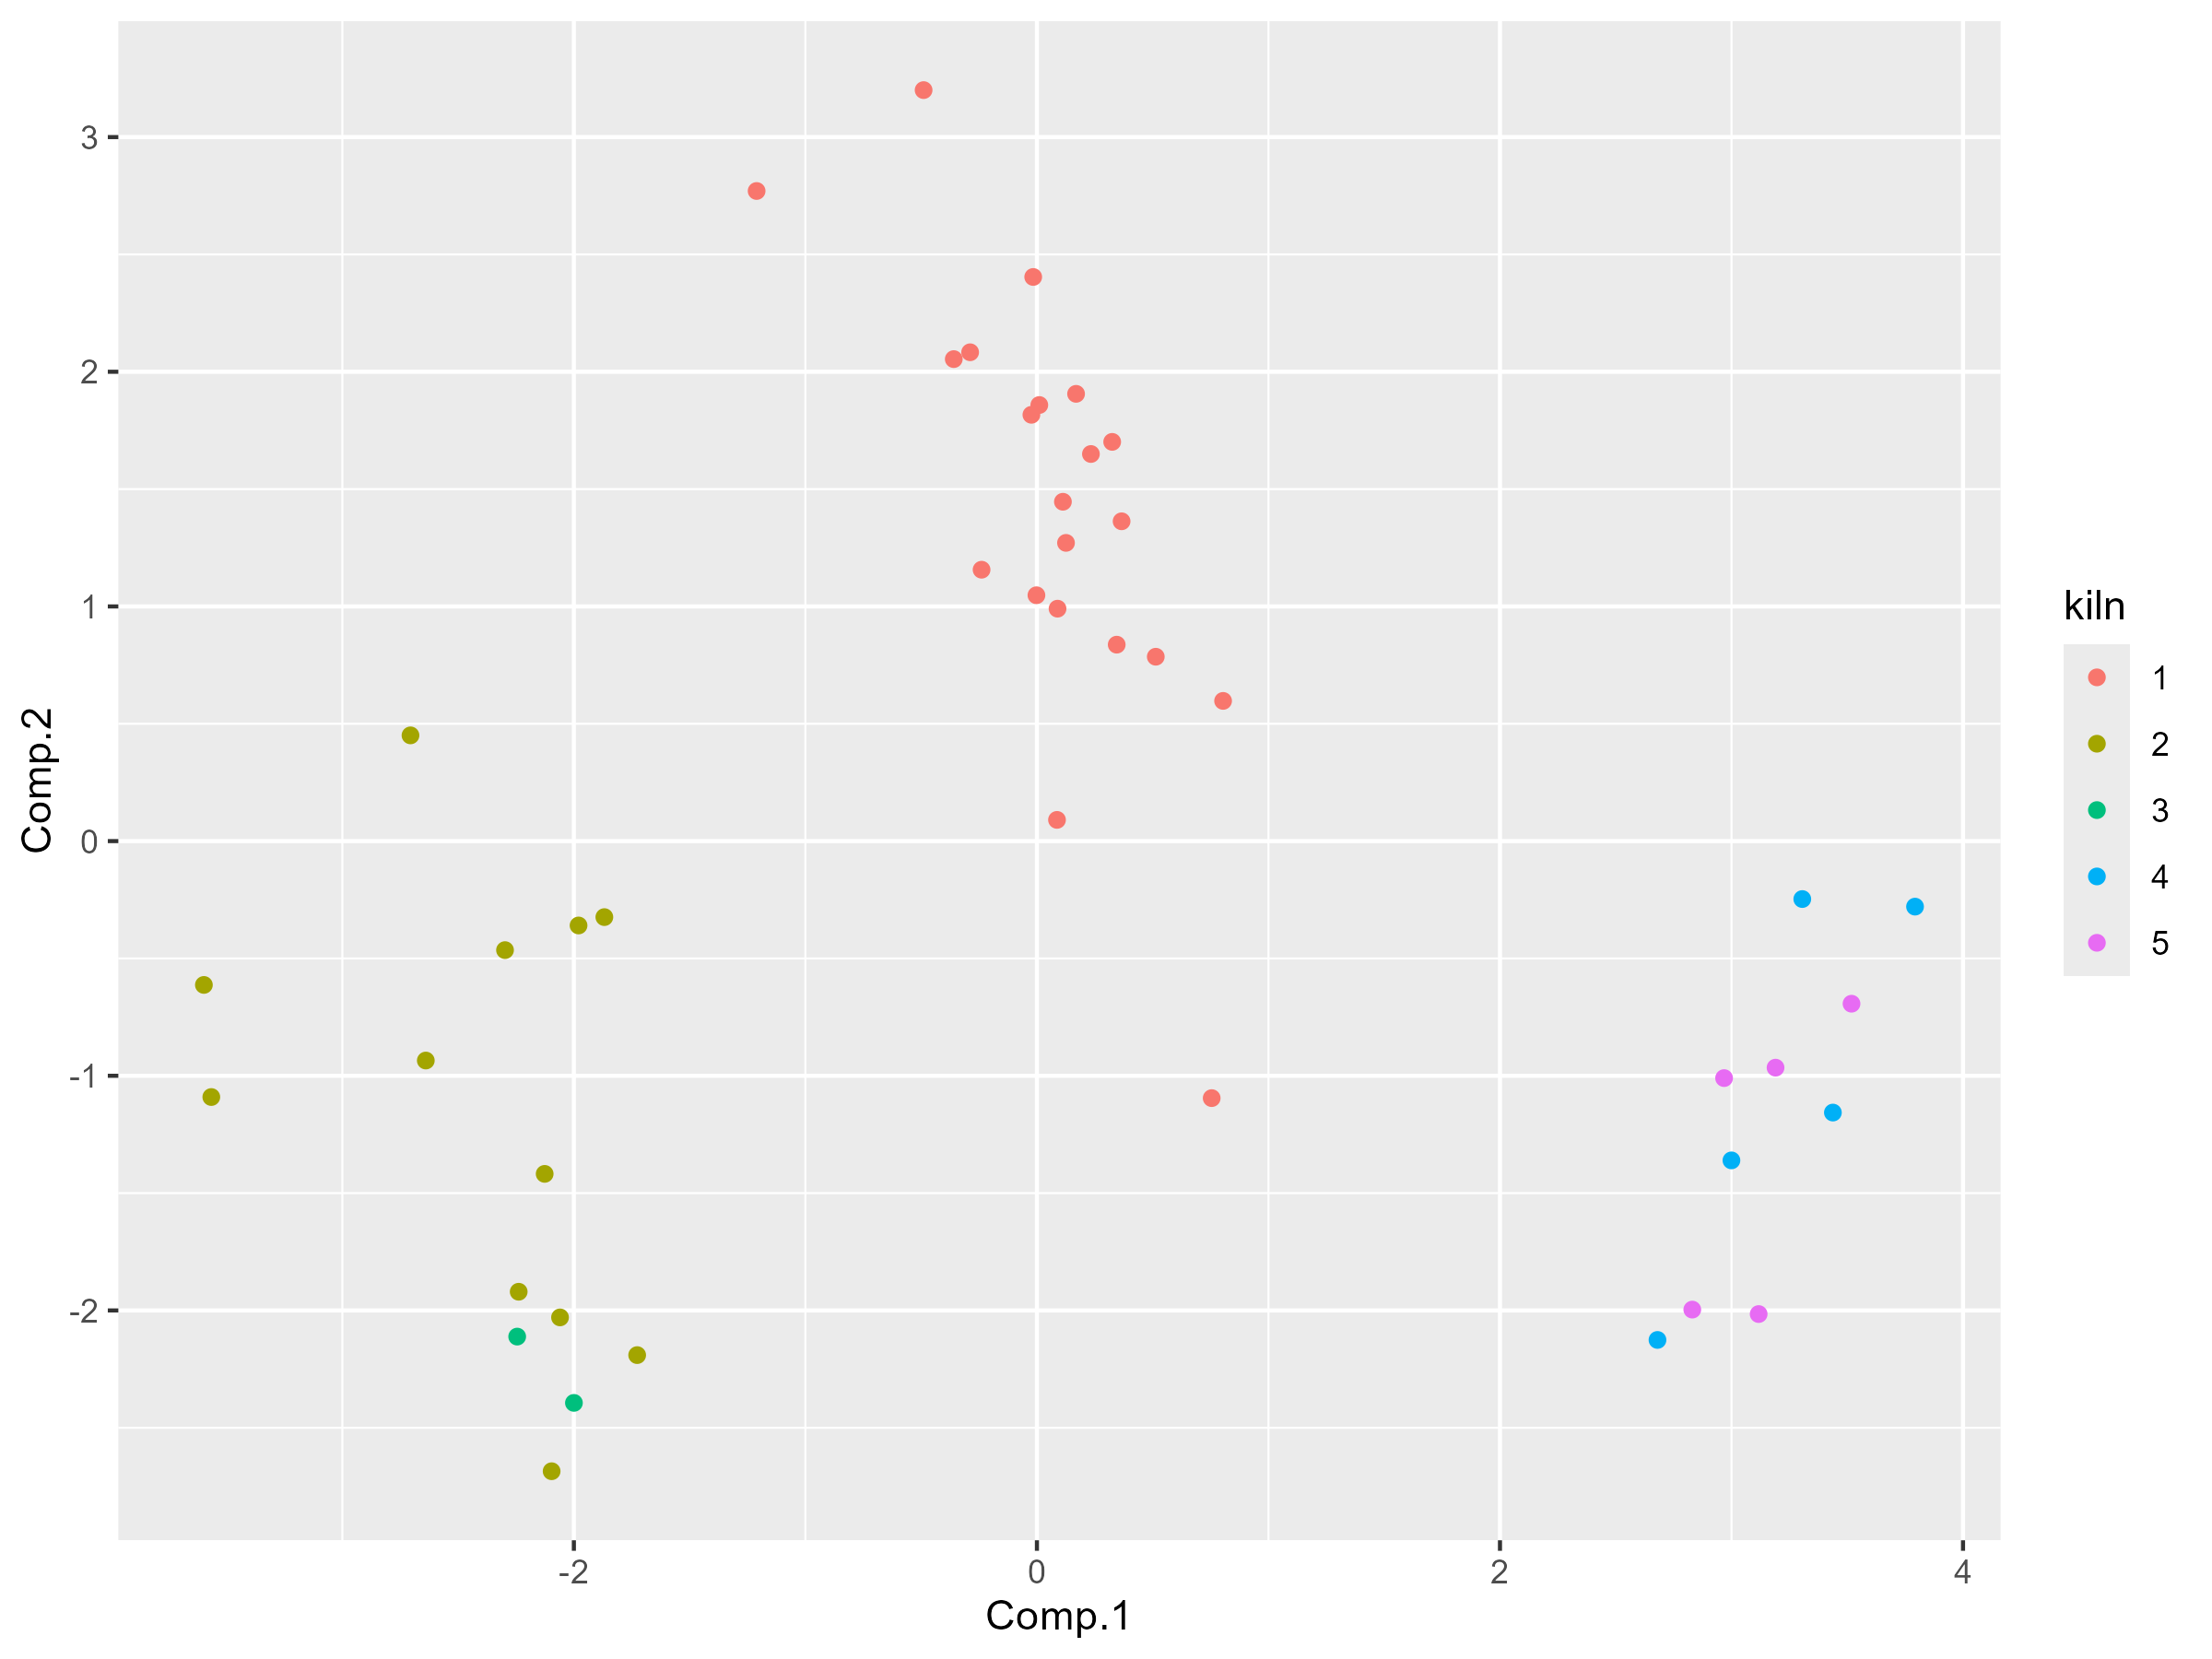
\includegraphics[width=0.6\textwidth]{../Figure/PCA_by_kiln.png}
		\caption{PCA 第一与第二主成分散点图(按窑口着色)}
		\label{fig:PCA_kiln}
	\end{figure}
	
	从图 \ref{fig:PCA_kiln} 中看出来,明显分成3组,恰好是5个窑所在的三个地区.
	
	用k均值聚类,对不同的类数计算解释百分比以确定分类个数:
	\begin{lstlisting}[language=R]
		## 对不同的类数计算解释百分比
		elbow_plot <- function(
		data,
		max_k = min(ncol(data), 10)) {
			rat <- numeric(max_k)
			rat[1] <- 0
			for (k in 2:max_k) {
				rkm <- kmeans(
				data,
				centers = k,
				nstart = 20
				)
				rat[k] <- (1 - rkm$tot.withinss / rkm$totss) * 100
			}
			plot(rat,
			xlab = "类数", ylab = "离差平方和解释百分比",
			type = "b"
			)
		}
	\end{lstlisting}
	\begin{figure}[H]
		\centering
		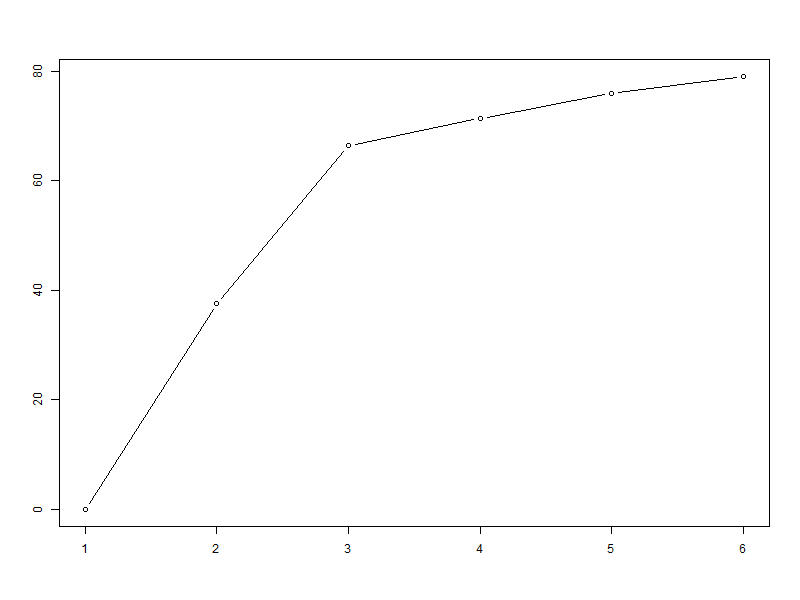
\includegraphics[width=0.6\textwidth]{../Figure/elbow_plot.png}
		\caption{不同聚类数 $k$ 下的 WSS 值(Elbow 图)}
		\label{fig:elbow}
	\end{figure}
	
	从图 \ref{fig:elbow} 中可见,分成3类以后再增加分类的效益明显降低.
	
	作k均值聚类,结果见附录输出 \ref{lst:Kmean} .
	\begin{lstlisting}[language=R]
		## 作k均值聚类
		pot_km <- kmeans(pottery_scale[, 1:9],
		centers = 3, nstart = 20
		)
	\end{lstlisting}
	
	按各类中心的变量值对类别重新编号,这样可以使得聚类的编号有稳定结果:
	\begin{lstlisting}[language=R]
		## 按各类中心的变量值对类别重新编号
		cluster_reorder <- function(
		data, km_res,
		label = rownames(data)) {
			xrmean <- rowMeans(data)
			clus_old <- km_res$cluster
			names(clus_old) <- label
			clus_new <- clus_old
			clus_new[] <- as.integer(fct_reorder(
			factor(clus_old), xrmean, mean,
			.desc = TRUE
			))
			clus_new
		}
		clus_new <- cluster_reorder(
		pottery_scale[, 1:9],
		pot_km,
		label = pottery_scale[["kiln"]]
		)
	\end{lstlisting}
	
	对比kiln和clus\_new的值:
	\begin{lstlisting}[language=R]
		## 对比kiln和clus_new的值:
		table(clus_new, pottery_scale[["kiln"]])
		# clus_new  1  2  3  4  5
		#        1 21  0  0  0  0
		#        2  0 12  2  0  0
		#        3  0  0  0  5  5
	\end{lstlisting}
	
	可以看出,分类1由1号窑组成,分类2由2、3号窑组成,分类3由4、5号窑组成.
	
	最后,按照分类作主成分图,见图 \ref{fig:PCA_cluster} .
	\begin{lstlisting}[language=R]
		## 按分类作主成分图:
		as_tibble(pot_pca) |>
		mutate(cluster = factor(clus_new)) |>
		ggplot(aes(
		x = Comp.1, y = Comp.2, color = cluster
		)) +
		geom_point() -> p3
	\end{lstlisting}
	\begin{figure}[H]
		\centering
		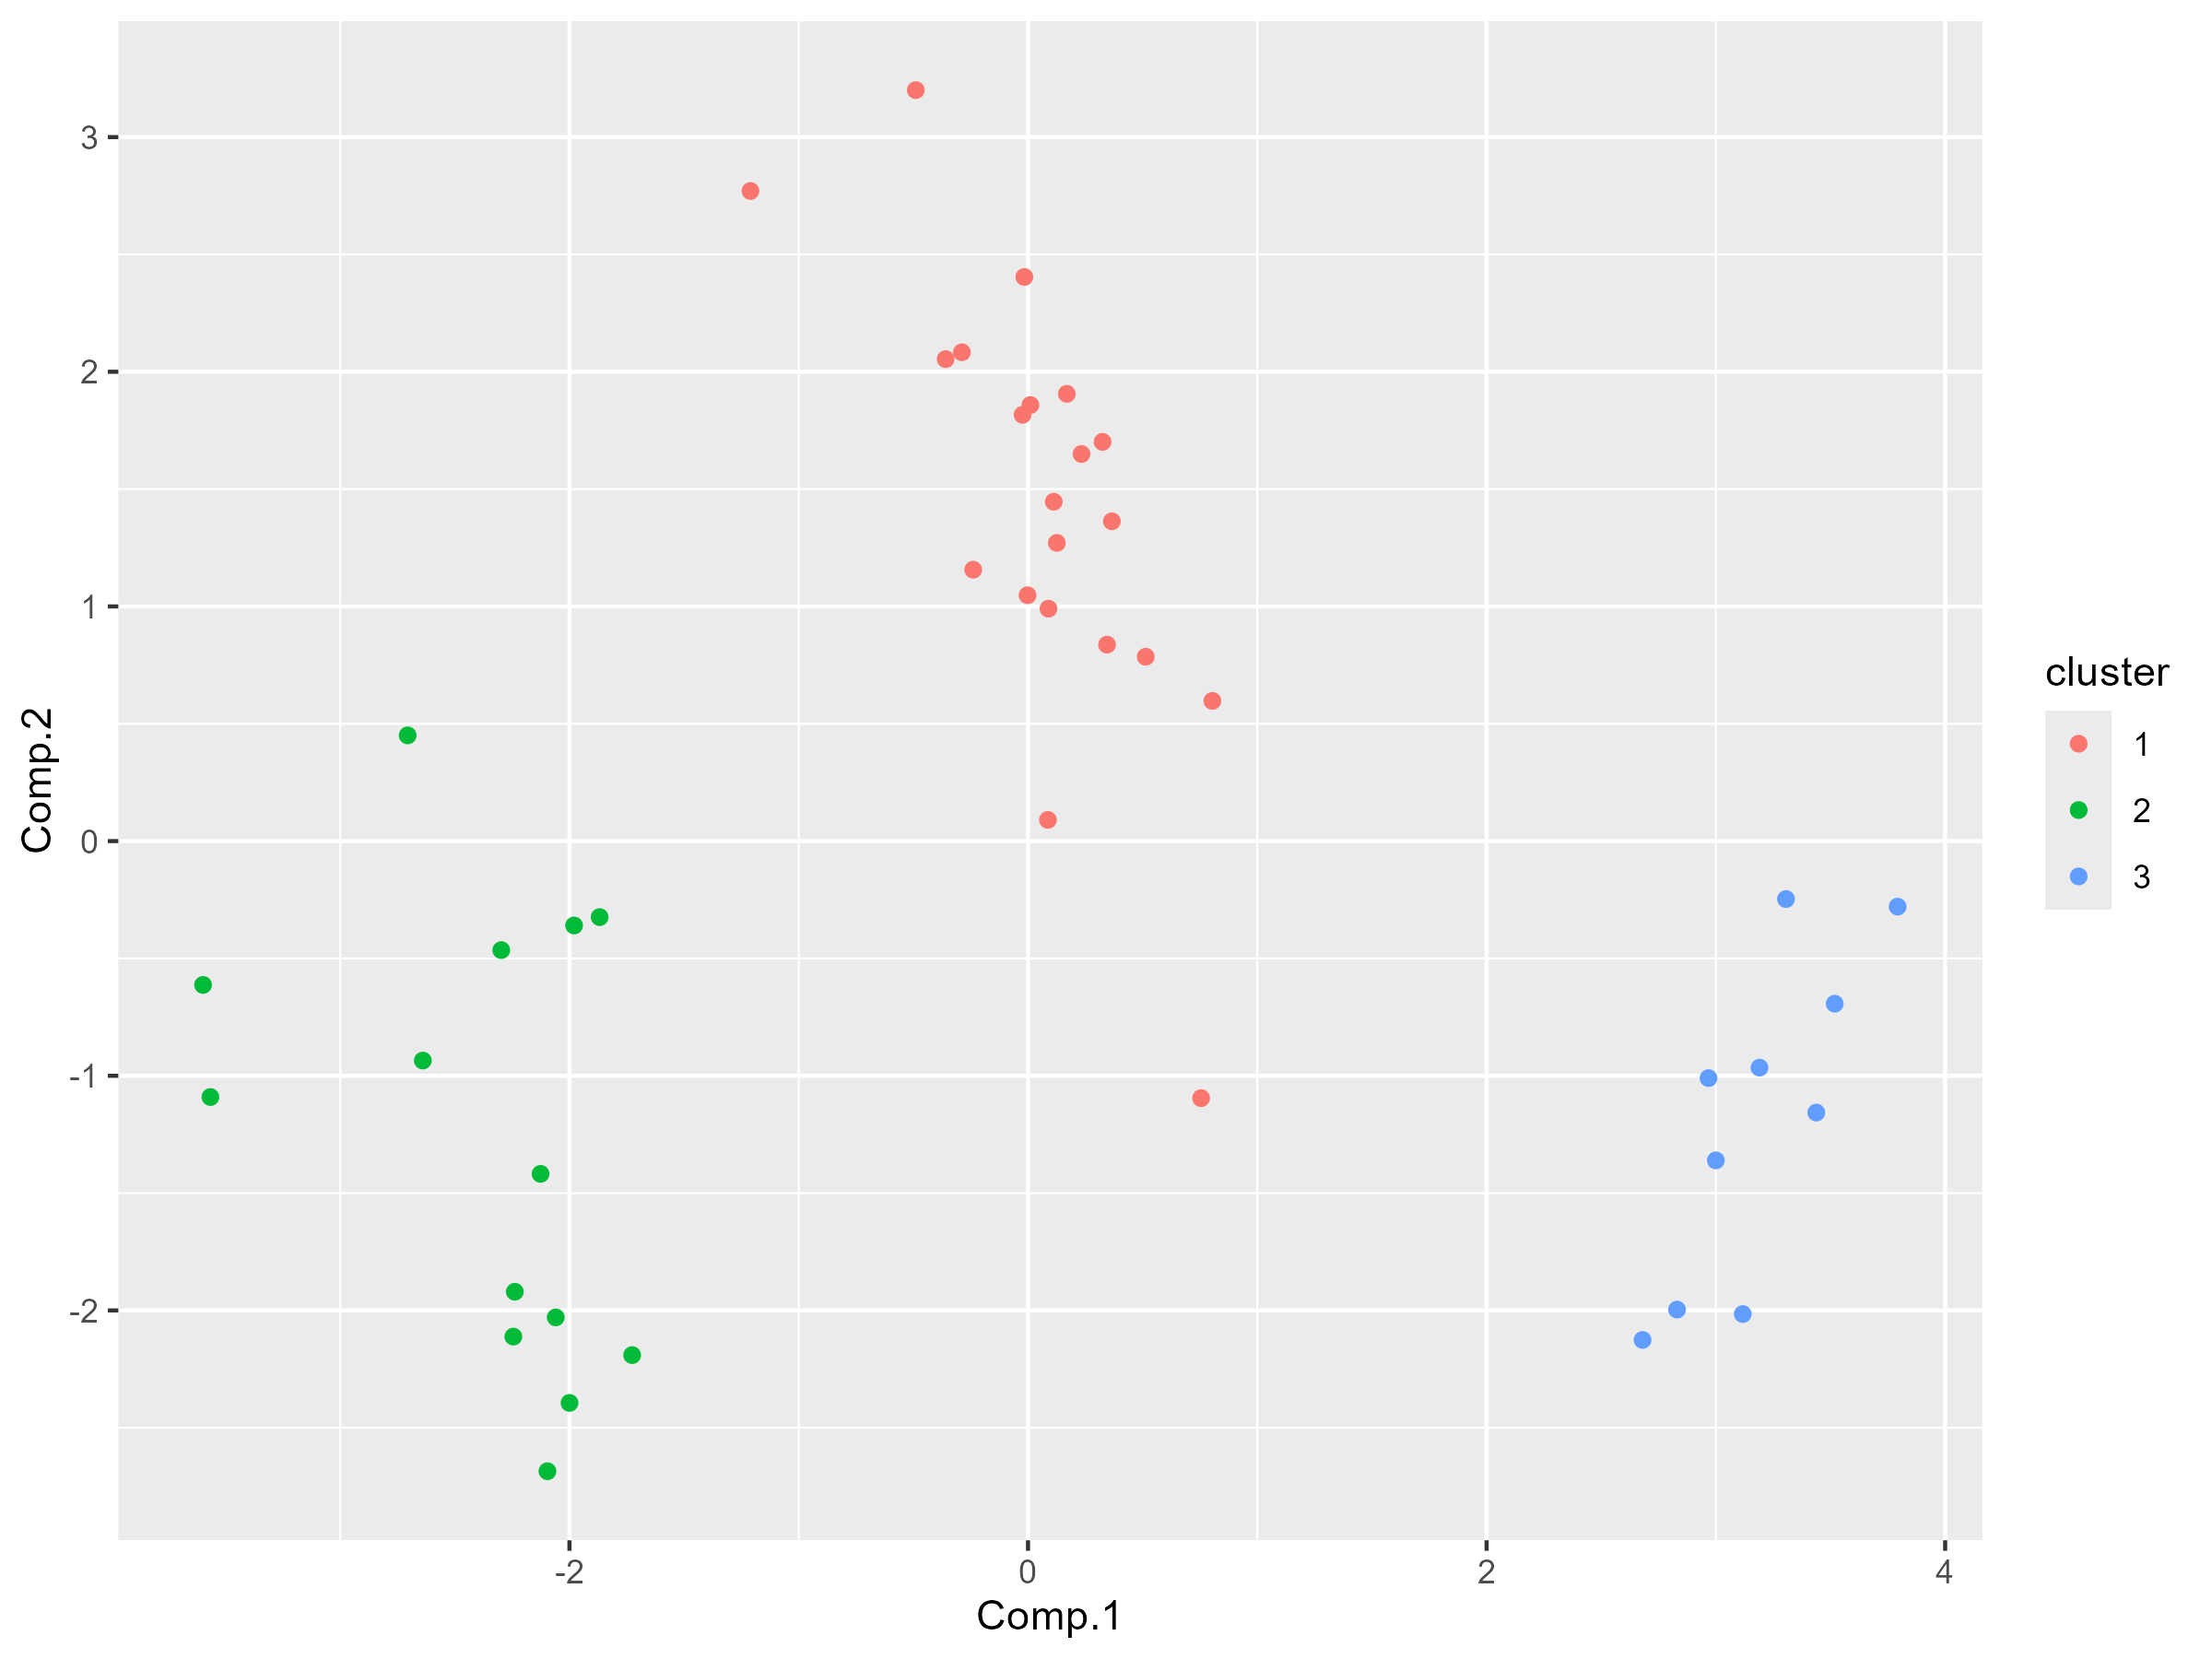
\includegraphics[width=0.6\textwidth]{../Figure/PCA_by_cluster.png}
		\caption{PCA 主成分散点图(按聚类结果着色)}
		\label{fig:PCA_cluster}
	\end{figure}
	\newpage
	
	\begin{thebibliography}{99}
		\bibitem{a}李高荣,吴密霞 编著. \emph{多元统计分析}[M]. 北京: 科学出版社, 2021.
		\bibitem{b}高惠璇. \emph{应用多元统计分析}[M].北京大学出版社, 2005.
		\bibitem{c}费宇. \emph{多元统计分析:基于R}[M].中国人民大学出版社, 2014.
	\end{thebibliography}
	
	\newpage
	
	\begin{appendices}
		\renewcommand{\thesection}{\Alph{section}}
		\section{部分程序输出}
		\begin{lstlisting}[language=R, caption={K均值聚类结果}, label=lst:Kmean]
			K-means clustering with 3 clusters of sizes 10, 21, 14
			
			Cluster means:
			Al2O3      Fe2O3       MgO        CaO        Na2O        K2O       TiO2
			1  0.7551242 -1.7225881 -1.061037 -1.0446359 -1.07655028 -1.3826254  0.7971355
			2  0.4477072  0.6951290 -0.370851  0.9366328  0.57687920 -0.1139204  0.3389812
			3 -1.2109353  0.1877267  1.314160 -0.6587807 -0.09635432  1.1584702 -1.0778543
			MnO        BaO
			1 -1.43823665 -0.1714027
			2  0.01349852  0.2118580
			3  1.00706411 -0.1953565
			
			Clustering vector:
			1  2  3  4  5  6  7  8  9 10 11 12 13 14 15 16 17 18 19 20 21 22 23 24 25 26
			2  2  2  2  2  2  2  2  2  2  2  2  2  2  2  2  2  2  2  2  2  3  3  3  3  3
			27 28 29 30 31 32 33 34 35 36 37 38 39 40 41 42 43 44 45
			3  3  3  3  3  3  3  3  3  1  1  1  1  1  1  1  1  1  1 
			
			Within cluster sum of squares by cluster:
			[1] 27.71633 55.91185 49.30545
			(between_SS / total_SS =  66.4 %)
			
			Available components:
			
			[1] "cluster"      "centers"      "totss"        "withinss"     "tot.withinss"
			[6] "betweenss"    "size"         "iter"         "ifault"
		\end{lstlisting}
	\end{appendices}
	
\end{document}